% Created 2010-06-15 Tue 22:01
\documentclass[11pt]{article}
\usepackage[utf8]{inputenc}
\usepackage[T1]{fontenc}
\usepackage{graphicx}
\usepackage{longtable}
\usepackage{float}
\usepackage{wrapfig}
\usepackage{soul}
\usepackage{amssymb}
\usepackage{hyperref}
\usepackage{graphicx}

\title{Katana: A Userland Toolchain-Oriented Hotpatching System}
\author{James Oakley}
\date{15 June 2010}

\begin{document}

\maketitle

\setcounter{tocdepth}{3}
\tableofcontents
\vspace*{1cm}


\section{Introduction}
\label{sec-1}

  Katana aims to provide a hot-patching system for userland. Further
  it aims to work with existing toolchains and formats so as to be
  easy to use and to hopefully pave the way for incorporating patching
  as a standard part of the toolchain. Because of this aim, Katana
  operates at the object level rather than requiring any access to the
  source code itself. This has the added bonus of making it, in
  theory, language agnostic (although no work has been done to test it
  with anything besides programs written in C). A diagram of software
  lifecycle with hotpatching is shown below


\begin{figure}[h!]
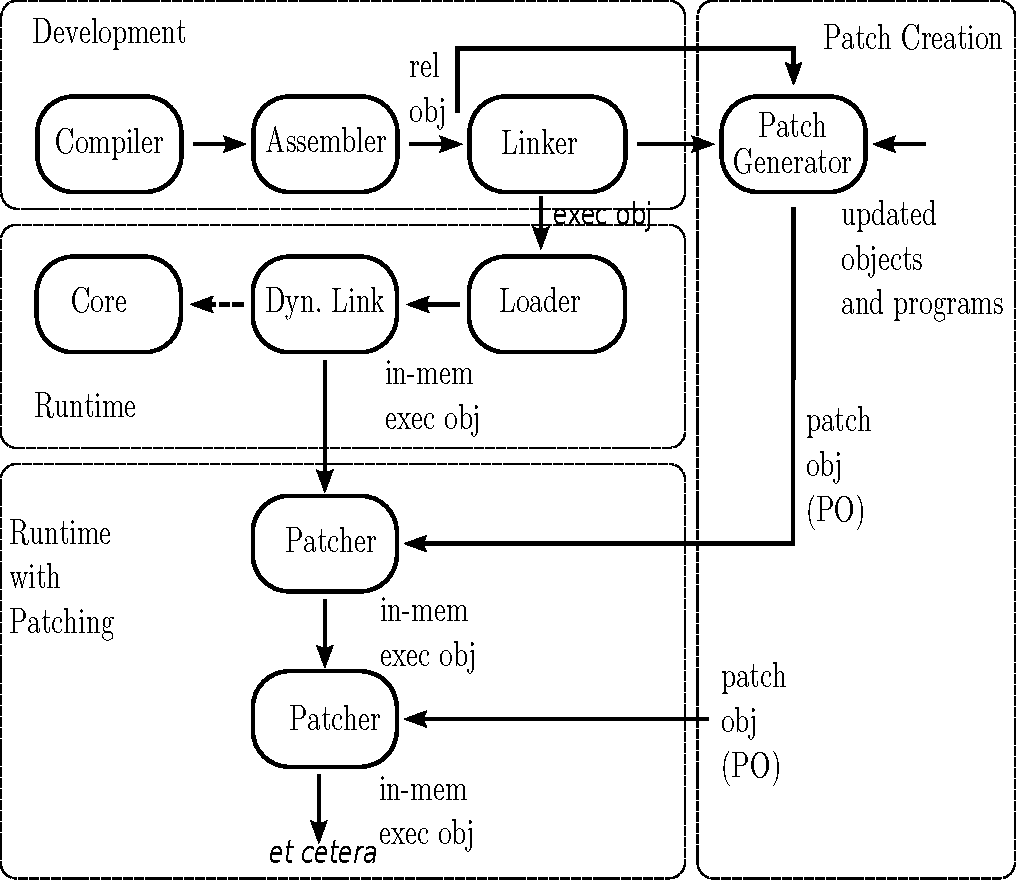
\includegraphics[width=3in]{./softwarelifecycle.pdf}
\end{figure}


  This document is intended to provide a users guide to Katana,
  insight into its inner workings, and discussion of its flaws and
  plans for the future. As the software is not complete, making use of
  Katana without understanding the inner workings and technical
  shortcomings is not recommended. Nevertheless, the only sections of
  this document necessary for ``Users' Guide'' purposes are 
  \hyperref[sec-3]{``What Katana Does''}, \hyperref[sec-4]{``What Katana Does Not Do (Yet)''}, and most importantly 
  \hyperref[sec-6]{``How to Use Katana''}.
 
  This document is a work in progress. It is not a polished guide yet.
\section{Other Systems}
\label{sec-2}

  There are other hotpatching systems in existence. The curious are
  invited to explore Ginseng and Polus. Both of these systems parse
  the source code, which adds significant complexity to them and
  results in significant programmer annotation of the code to give
  hints to the systems. Ginseng uses complicated type-wrappers
  when patching variables which does not fit cleanly with existing
  executables and has some impact on the performance of the
  software. Ginseng is considerably more mature than Katana,
  however. Neither system is production ready, but Ginseng is probably
  closer than Katana at the moment.

  The system most like Katana in many ways is KSplice, and the curious
  reader is definitely invited to investigate. KSplice patches the
  kernel and not userland, does not attempt to patch variables, and
  creates patches as kernel modules rather than working towards a
  general ELF-based patch format.
\section{What Katana Does}
\label{sec-3}

\begin{itemize}
\item Runs on x86 and x86-64
\item Generates patches for simple programs
\item Applies simple patches
\end{itemize}
\section{What Katana Does Not Do (Yet)}
\label{sec-4}

\begin{itemize}
\item Patch any major programs: it has not yet been demonstrated on
    anything more than toy examples
\item Provide any method to handle opaque data it cannot patch (void*,
    situations where which action a user would prefer is unclear, etc)
\item Patch previously patched processes
\item Provide robust operation
\item Run on any architectures other than x86 and x86-64
\item Tested on any operating system besides Linux
\item Allow for calls in patched code to previously unused functions
\item Work for programs which actually make use of some of the large
    code model features of the x86-64 ABI.
\item And much more
\end{itemize}
  See \hyperref[sec-10]{Roadmap} for more things which are not complete

\section{What Katana May Never Do}
\label{sec-5}

\begin{itemize}
\item Work on any binary formats besides ELF
\end{itemize}
\section{How to Use Katana}
\label{sec-6}

  Katana is intended to be used in two stages. The first stage
  generates a patch object from two different versions of an
  treee. By an object tree, we mean the set of object files (.o files)
  and the executable binary they comprise. Katana works completely at
  the object level, so the source code itself is not strictly
  required, although all objects must be compiled with debugging
  information. This step may be done by the software vendor. In the
  second stage, the patch is applied to a running process. The
  original source trees are not necessary during patch application, as
  the patch object contains all information necessary to patch the
  in-memory process at the object level. It is also possible to view
  the contents of a patch object in a human-readable way for the
  purposes of sanity-checking, determining what changes the patch
  makes, etc.
\subsection{Preparing a Package for Patching Support}
\label{sec-6.1}

   Katana aims to be much less invasive than other hot-patching system
   and require minimal work to be used with any project. It does,
   however, have some requirements.\\
   Required CFLAGS:
\begin{itemize}
\item -g
\end{itemize}
   Recommended CFLAGS:
\begin{itemize}
\item -ffunction-sections
\item -fdata-sections
\end{itemize}
   Recommended LDFLAGS:
\begin{itemize}
\item --emit-relocs
\end{itemize}
\subsection{To Generate a Patch}
\label{sec-6.2}

   Let the location of your project be /project. You must have two
   versions of your software available: the version identical to the
   running software which must be hotpatched, call it v0, and the
   version to which you wish to hotpatch the running software, call it
   v1. Let foo be the name of your program. Then /project/v0/foo must
   exist and /project/v0 must also contain (possibly in
   subdirectories) all of the object files which contributed to
   /project/v0/foo. The source code itself is immaterial, as Katana
   does not parse it. Similarly, /project/v1/foo must exist and
   /project/v1 contain all of the object files contributing to
   /project/v1/foo. Katana is then invoked as

   \texttt{katana -g [-o OUTPUT\_FILE] /project/v0 /project/v1 foo}

   or more formally

   \texttt{katana -g [-o OUTUT\_FILE] OLD\_OBJECTS\_DIR NEW\_OBJECTS\_DIR EXECUTABLE\_NAME}

   If \texttt{-o OUTPUT\_FILE} is not specified, the output file will be \texttt{OLD\_OBJECTS\_DIR/EXECUTABLE\_NAME.po}
\subsection{To Apply a Patch}
\label{sec-6.3}

   The process to be patched is running with a pid of PID. It can be
   patched from its current version to a more recent version by the
   Patch Object (PO) file PATCH. Katana is then invoked as

   \texttt{katana -p [-s] PATCH PID}

   If all goes well, the patcher will run, print out some status
   messages, and leave your program in better state than it found
   it. The optional -s flag tells Katana to stop the target program
   after patching it and detaching from it. This is mostly of use for
   debugging Katana.
\subsection{To View a Patch}
\label{sec-6.4}

   One of the goals of Katana and its Patch Object (PO) format is to
   increase the transparency of patches: a user about to apply a patch
   should know what it will do. This goal is not yet fully realized,
   but it is possible to view some information about a patch with

   \texttt{katana -l PATCH}
\subsection{See Also}
\label{sec-6.5}

   the katana manpage (once it's written, which it is not yet)
\section{Patch Object Format}
\label{sec-7}

  This section of the document is not yet written. It will provide a description and specification of the PO format used by Katana
\section{Patch Generation Process}
\label{sec-8}

  This section of the document is not yet written. It will provide a
  description of the internal process that Katana uses to generate a
  patch. Understanding it is not necessary for using Katana.
\section{Patch Application Process}
\label{sec-9}

  This section of the document is not yet written. It will provide a
  description of the internal process that Katana uses to apply a
  patch. Understanding it is not necessary for using Katana.
\section{Roadmap}
\label{sec-10}

  This section is highly incomplete. Future goals include
\begin{itemize}
\item Better interaction with the heap and dynamically allocated variables
\item Better interaction with void*
\item More efficient use of .rodata
\item Patching already patched processes
\item Patch composition
\item Patch safety checking: make sure a patch actually corresponds to
    the process it's being applied to
\item Storing warnings from generation inside a patch
\end{itemize}

\end{document}